\documentclass[a4paper,10pt]{scrartcl}
\usepackage[utf8]{inputenc}
\usepackage[ngerman]{babel}
\usepackage[T1]{fontenc}
\usepackage{lmodern}	% das ist bei Carsten nötig, sonst ist die Schrift verpixelt.
\usepackage{a4wide}
\usepackage{graphicx}

\usepackage{xcolor}
\usepackage[pdftex]{hyperref}
\hypersetup{
    pdftitle = {Fallstudie: Steuerungs- und Regelungsentwurf},
    colorlinks = true,
    linkcolor={red!20!black},
    citecolor={blue!50!black},
    urlcolor={blue!80!black},
}

\newcommand{\figref}[1]{Abb.~\ref{#1}} 

\newcommand{\tcred}[1]{\textcolor{red}{#1}} % für tmp-Hervorhebungen
\newcommand{\tcblue}[1]{\textcolor{blue}{#1}} % für tmp-Hervorhebungen





% Title Page
\title{RST-Versuchsstände  -- Aufbau und aktuelle Ergebnisse}
\subtitle{Entwurf}
\author{Robert Heedt, Carsten Knoll, Jan Winkler}


\begin{document}
\maketitle

\section*{Kurzzusammenfassung}
\begin{abstract}
Dieser technische Bericht beschreibt einige Versuchsstände am Institut für Regelungs- und Steuerungstheorie.
Ziel ist es, einen Überblick über ihren grundlegenden Aufbau, ihre Funktionsweise und die experimentellen Möglichkeiten zu geben.
\end{abstract}

\section{Wagen-Pendel-System}



\subsection{Hardware-Aufbau} 

Der in Abbildung \ref{fig_3fachpendel_foto} dargestellte Versuchsstand wurde von der Firma Hassomed \cite{Hassomed} hergestellt.
Er besteht aus einer Schiene der Länge $4.5$m auf der ein Schlitten gleitet, welcher über einen Zahnriemen von einem Synchron-Motor angetrieben wird.
Am Schlitten ist ein Dreifachpendel angebracht. Zur Erfassung der Gelenkwinkel sind Inkrementalgeber verbaut. Die Messwerte werden in den Hohlwellen der Achsen optisch übertragen, sodass die drei Drehgelenke unbeschränkt rotieren können. 
\begin{figure}[h!]
\begin{center}
\includegraphics[width=.8\textwidth]{img/3fach_pendel_klein.jpg}
\end{center}
\caption{Aufbau des Versuchsstandes. Komponenten: Steuerungs-PC, sbRIO (Echtzeit-PC+FPGA), Leistungselektronik, Schiene, Synchron-Mototor, Schlitten, drei Pendelarme.}
\label{fig_3fachpendel_foto}
\end{figure}


\subsection{Softwarekomponentenarchitektur }

\begin{figure}[ht]
    \begin{center}
    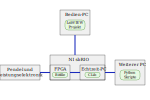
\includegraphics[width=.8\textwidth]{img/pendel_hw_sw}
    \end{center}
    \caption{Verteilung der Softwarekomponenten auf Hardware.}
    \label{fig_hw_sw}
\end{figure}

Der Code zum Betrieb des Versuchsstandes verteilt sich auf mehrere Ebenen, die sich aus unterschiedlicher Hardware und verwendeter Software zusammensetzen, siehe Abb.~\ref{fig_hw_sw}. Das Fundament bildet LabVIEW auf einem herkömmlichen PC, da von National Instruments die Hardware-Schnittstelle softwareseitig gut unterstützt wird. Hier werden Messsignale vorverarbeitet - beispielsweise die Inkrementimpulse gezählt - das Stellsignal ausgegeben und Systemgrößen live visualisiert. Zeitkritische Logik führt das FPGA mit einer hohen Abtastrate aus.

Regler und Beobachter wurden in C als Shared Library -- nachfolgend \emph{CLib} genannt -- geschrieben, die in das LabVIEW-Projekt eingebettet auf dem Echtzeit-PC mit 500 Hz Abtastrate ausgeführt wird. Dieses Vorgehen hat mehrere Vorteile:

\begin{enumerate}
    \item Änderungen der Reglerlogik kompilieren in wenigen Sekunden; es muss kein FPGA Layout generiert werden, was in der Größenordnung einer halben Stunde dauert
    \item CLib kann ohne LabVIEW getestet und simuliert werden
    \item prozedurale Logik und textbasierte Entwicklung subjektiv komfortabler
\end{enumerate}

Zudem stellt die CLib einen Netzwerksocket bereit, über den Befehle an den Regler gesendet und Messwerte abgefragt werden können. Diese Schnittstelle ermöglicht es etwa, längere Messreihen komplett zu automatisieren.

Eine ausführlich dokumentierte Sammlung von Python-Skripten garnieren den Software-Stapel. Darunter befinden sich Tools zur Reglerdimensionierung, Trajektorienplanung, Messdatenauswertung und Simulation. Auch das Training für Bestärkendes Lernen findet auf dieser Schicht statt.

% \subsection{Modell und Systemparameter }
% Eventuell nachtragen

\subsection{Sicherheitsfeatures}

Der Betrieb des Versuchsstandes wird wieder auf mehreren Ebenen mit verschiedenen Methoden abgesichert. In der CLib werden Ist- und Sollzustand der Systemgrößen ständig miteinander verglichen. Kommt eine Heuristik zum Schluss, dass der Regler das System nicht mehr im Griff hat, wird in einen Tranquilisierungsmodus umgeschaltet. Das Ziel ist jetzt, dem Pendel sanft Energie zu entziehen, bis es wieder in der unteren Ruhelage verharrt. Dieser Modus wurde als Impedanzregelung entworfen; anschaulich bedeutet das, der Wagen bewegt sich so, als wäre er durch eine gedämpfte Feder mit dem Mittelpunkt der Schiene verbunden. Der Wagen fügt sich also zu einem gewissen Grad der Bewegung der frei rotierenden Pendelarme, durch die virtuelle Dämpfung nimmt deren Intensität aber nach und nach ab. Brenzlig wird es, wenn der Wagen mit hoher Geschwindigkeit in die Nähe des Schienenendes rast. Für diesen Fall nimmt die virtuelle Federkonstante abhängig von der Wagenposition stark zu, so wird er eindrücklich Richtung Mitte forciert.

Scheitert all das, so greift die LabVIEW-Ebene ein, die bei ausgelöstem Endlagenschalter den Motor hart stoppt. Schlägt auch das fehl, sind an den Enden der Schiene schlussendlich hydraulische Dämpfer montiert.

Die Kombination aller Mechanismen hat die Konsequenz, dass auch riskante Experimente wie selbstständiges Durchführen von Episoden des Bestärkenden Lernens mit geringem Verschleiß, Beschädigungsrisiko und Überwachungsaufwand durchgeführt werden können. Insbesondere die automatische Tranquilisierung verringert aufgrund ihres Wirkprinzips den mechanischen Verschleiß, weil keine abrupten Beschleunigungen entstehen.

\subsection{Bisherige Ergebnisse}

Zunächst wurden basierend auf dem Systemmodell ein linearer LQR-Entwurf für alle acht Ruhelagen durchgeführt und experimentell erprobt. Dabei zeigte sich sowohl die prinzipielle Tauglichkeit des Systems, als auch die erwarteten Robustheitsunterschiede: Das Ausmaß an Störungen (z.\,B. Kraftstoß auf den äußeren Pendelarm), welches vom rückgeführten System noch stabilisiert werden kann hängt von der jeweiligen RL ab und ist in "`\texttt{OOO}"' am geringsten.
    
\medskip
    
Zwischen den Ruhelagen können offline Übergänge berechnet werden. Dabei werden unter Nutzung des Systemmodells durch Optimierung Vorsteuerung und Rückführung ermittelt.
Eine derartig ermittelte Überführung ist in Abbildung~\ref{fig:uoo_ooo} dargestellt.
Ist kein direkter Übergang möglich, werden mehrere funktionierende Übergänge verkettet um das Ziel zu erreichen; auf Wunsch auch automatisch. So ist reproduzierbar jede Ruhelage als Startpunkt für die Evaluation von Regelungsalgorithmen möglich.

\medskip
Bestärkendes Lernen wurde bisher in zwei Szenarien erfolgreich getestet: dem seitlichen Versetzen des Dreifachpendels in unterer Position und dem Aufschwingen des Einfachpendels\footnote{Als Alternative zum den in \figref{fig_hw_sw} gezeigten drei Pendelarmen kann ein ca. 1m langes Einfachpendel montiert montiert werden}. Sämtliche Trainingsdaten stammen aus Experimenten am Versuchsstand; um die große Menge an Messdaten aufzunehmen musste die Durchführung möglichst komfortabel werden. Eine Trainingsepisode besteht aus dem Generieren einer Trajektorie, dem Ausführen derselben auf dem Versuchsstand, dem Extrahieren relevanter Messdaten und dem Training des gelernten Modells mit dem neuen Wissen. Diese Iteration wurde inzwischen voll automatisiert, sodass im besten Fall ein Mitarbeiter nur im Notfall eingreifen muss.

\begin{figure}
    \centering
    \includegraphics[scale=0.7]{img/uoo_ooo_3.0_around.csv.pdf}
    \caption{Aufschwingen von der Ruhelage uoo nach ooo.}
    \label{fig:uoo_ooo}
\end{figure}
    

\subsection{Ausblick}

Folgende Arbeiten stehen bezüglich des Dreifachpendelversuchsstandes aus

\begin{itemize}
 \item Überarbeitung Bedienoberfläche zur manuellen Demonstration
 \item Experimentserie zum Bestärkenden Lernen z.\,B. auf Basis des Deep-Ensemble-Ansatzes
 (inkl. weiterer Experiment-Automatisierung)
\end{itemize}

    
\newpage

\section{Zweirädriger Balancier-Roboter}    
Das in \figref{fig_robo1} dargestellte einachsige Fahrzeug  besitzt zwei Einzelradantriebe (Gleichstromgetriebemotoren), einen STM32-Mikrokontroller und ein Akkumulator-Paket zuer Energieversorgung.


\begin{figure}[h]
    \begin{center}
    \includegraphics[width=.5\textwidth]{img/robo2_klein.jpg}
    \end{center}
    \caption{Balancier-Roboter.}
    \label{fig_robo1}
\end{figure}

\newpage
\section{Hubschrauberrack}
Der in in \figref{fig_helirack1} dargestellte Helikopterversuchsstand besitzt zwei Rotoren (bürstenlose Gleichstrommotoren), einen STM32-Mikrokontroller und ein Akkumulator-Paket zuer Energieversorgung.

\begin{figure}[ht]
    \begin{center}
    \includegraphics[width=.8\textwidth,trim=0 2mm 0 5.5mm, clip]{img/heli_klein.jpg}
    \end{center}
    \caption{Helicopter-Rack.}
    \label{fig_helirack1}
\end{figure}


\newpage

    
\renewcommand\refname{Referenzen}
\begin{thebibliography}{}
  \bibitem{Hassomed}
  \textsc{Hassomed GmbH}: \textit{Produktbeschreibung Dreiarmpendel}, \url{https://hasomed.de/produkte/dreiarm-pendel/}


\end{thebibliography}

\end{document}          
